
%il reste à faire une partie sur les applications affines

Notre méthode de traitement des homographies repose sur la décomposition d'une homographie qui permet d'interpréter cette dernière en terme de mouvement de caméra. La partie ci-dessous présente cette décomposition.





\ssse{Changement d'orientation de caméra :}
On étudie ici un cas a priori particulier d'homographie $h$   que l'on peut interpréter comme un mouvement de caméra (on montrera par la suite que c'est en fait un cas général).\\
\begin{figure}[h!]
\label{shmdecomp}
\centering
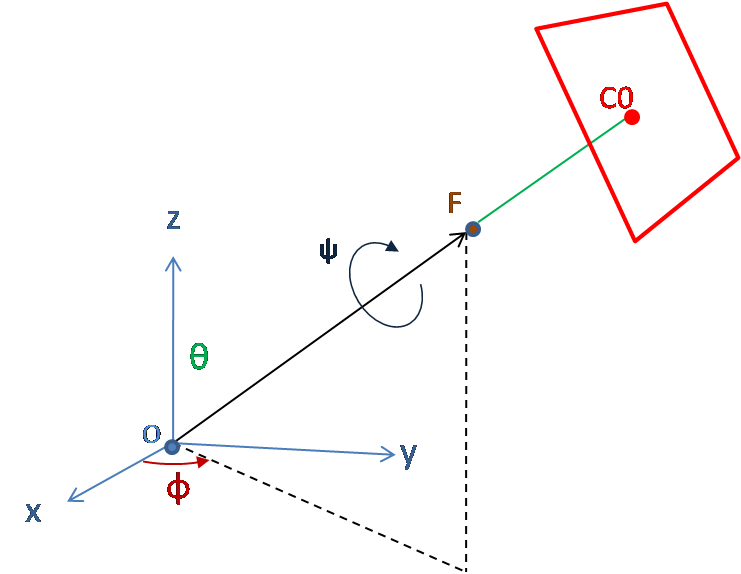
\includegraphics[width=10cm]{shema_decomp.png}

\caption{Illustration d'un mouvement de caméra $(X_v =0)$. $F$ représente le point focal de la caméra, le plan rouge est le plan image de la caméra.}
\end{figure}
\begin{Def}
Une homographie unidirectionnelle est une application $h:\mathbb{R}^{2} \mapsto \mathbb{R}^{2}$ définit par 
\begin{equation*}
h(x,y)=\left ( \frac{ax+p}{rx+t} , \frac{cy+p}{rx+t} \right)
\end{equation*}
Où $a,p,c,q,r,t$ sont des réels 
\end{Def}

\paragraph{Approche géométrique :}
On se place dans l'espace $\mathbb{R}^{3}$,on le munit d'une base orthonormale directe $(x_{0},y_{0},z_{0})$,\\ l'image de départ sera située dans le plan $P_{1}= \mathbb{R}^{2}\times \{0\}$.\\
On doit maintenant positionner notre caméra par rapport à l'image de départ \ref{shmdecomp}.
\begin{itemize}
\item On note $F$ la position de l'objectif de la caméra, et $w$ le vecteur directeur unitaire de l'axe optique de la caméra. L'axe optique de la caméra est donc la droite passant par $F$ et dirigée par $w$.
\item On note $\delta$ la distance entre l'objectif et l'écran.
\item L'écran $P_{2}$ est alors le plan affine passant par $F+\delta w$ et perpendiculaire à l'axe optique de la caméra.
\begin{equation*}
P_{2}=\{Y\in \mathbb{R}^{3}|(Y-F-\delta w)\cdot w=0\}=\{Y\in \mathbb{R}^{3}|(Y-F)\cdot w=\delta\}
\end{equation*}
\end{itemize}

On définit l'application $H$ qui à un point $X\in P_{1}$ lui associe sa projection homographique sur $P_{2}$. C'est-à-dire que le point $H(X)$ est le point d'intersection entre la droite $D_{X}$ (passant par $X$ et $F$) et le plan $P_{2}$.\\

L'application $H$ est une application de $P_{1}'$ dans $P_{2}$. Pour construire une expression analytique du mouvement de caméra, on peut munir le plan $P_{1}$ de la base $(x_{0},y_{0})$, de même le plan affine $P_{2}$ peut être muni d'un repère orthonormé $(C,u,v)$ tel que la famille $(u,v,w)$ soit un base orthonormale directe de $\mathbb{R}^{3}$, et que le point $C$ soit un point quelconque de l'écran qui servira d'origine.\\

On peut repérer le point $C$ par rapport au centre de l'écran $C_{0}$, c'est-à-dire la projection orthogonale de l'objectif sur l'écran : $C_{0}=Z+\delta w$ et $C=C_{0}+c_{u}u+c_{v}v$.\\

On peut alors définir les bijections $i$ et $k$
\begin{itemize}
\item $i:\mathbb{R}^{2}\rightarrow P_{1}$ telle que $i((x,y))=xx_{0}+yy_{0}$
\item $k:P_{2}\rightarrow \mathbb{R}^{2}$ telle que $k(X)= ((X-C)\cdot u,(X-C)\cdot v)=((X-F)\cdot u-c_{u}, (X-F)\cdot v-c_{v})$
\end{itemize}
On pose alors 
\begin{equation*}
h=k\circ H \circ i
\end{equation*}
h est une application définie sur $\mathbb{R}^{2}$ privé d'une droite.
\begin{prop}
On peut factoriser $h$ sous la forme
\begin{equation}
h = \tau_{c} \circ z_{\frac{\delta}{\delta'}}  \circ R_{\psi} \circ h_{\theta,\delta'} \circ R_{\phi} \circ \tau_{x_{v}}
\label{formul_decomp}
\end{equation}
Où $R_{\alpha}$ est la rotation d'angle $\alpha$, $\tau_y$ la translation du vecteur $-y$ et $h_{\theta,\delta'}$ est l'homographie unidirectionnelle 
\begin{equation*}
h_{\theta,\delta'}(x',y')=\left(\frac{-cos(\theta)x'}{1-\frac{sin(\theta)}{\delta'}x'} ,\frac{-y'}{1-\frac{sin(\theta)}{\delta'}x'}\right)
\end{equation*}
\end{prop}


\begin{lem}
$\forall X \in P_1$
\begin{equation*}
H(X)=Z+\delta w+\delta \frac{(F-X)-\left((F-X)\cdot w\right) w}{w\cdot (F-X)}
\end{equation*}
\end{lem}

\begin{proof}
Comme $D_{X}=\{X+t(F-X)|t\in\mathbb{R}\}$, si $H(X)$ existe alors 
\begin{equation*}
\exists t_{X},H(X)=X+t_{X}(F-X)
\end{equation*}
Comme $H(X)\in P_{2}$ alors
\begin{equation*}
(H(X)-F)\cdot w =\delta
\end{equation*}
Et donc 
\begin{equation*}
t_{X}=1+\frac{\delta}{w\cdot(F-X)}
\end{equation*}
Finalement on en déduit que l'application $H$ est définie sur $P_{1}'=P_{1}\backslash \{Y\in P_{1}|w\cdot(F-Y)=0\}$ et 
\begin{equation*}
H(X)=Z+\delta w+\delta \frac{(F-X)-\left((F-X)\cdot w\right) w}{w\cdot (F-X)}
\end{equation*}
\end{proof}

\subparagraph{Introduction du point visé :}
On se place dans le cas où le vecteur $w$ n'appartient pas à $P_{1}$. Dans ce cas, on peut définir $X_{v}$  le point de $P_{1}$ visé par la caméra, c'est-à-dire le point d'intersection entre l' axe optique et le plan $P_{1}$.On obtient alors 
\begin{equation*}
X_{v}=F-\delta'w \text{ et }\delta'=\small{\left|\frac{F \cdot z_{0}}{w\cdot z_{0}} \right|}
\end{equation*}
On peut alors en déduire que l'application $H$ est définie sur \[P_{1}'=P_{1}\backslash \{Y\in P_{1}|\delta'+w\cdot(X_{v}-Y)=0\}\] et 
\begin{equation*}
H(X)=X_{v}+(\delta+\delta')w+\delta_{2}\frac{(X_{v}-X)-\left((X_{v}-X)\cdot w\right) w}{\delta'+w\cdot (X_{v}-X)}
\end{equation*}



\subparagraph{Formulation analytique :}

L'application $H$ est une application de $P_{1}'$ dans $P_{2}$. Pour construire une expression analytique du mouvement de caméra, on peut munir le plan $P_{1}$ de la base $(x_{0},y_{0})$, de même le plan affine $P_{2}$ peut être muni d'un repère orthonormé $(C,u,v)$ tel que la famille $(u,v,w)$ soit un base orthonormale directe de $\mathbb{R}^{3}$, et que le point $C$ soit un point quelconque de l'écran qui servira d'origine.

On peut repérer le point $C$ par rapport au centre de l'écran $C_{0}$, c'est-à-dire la projection orthogonale de l'objectif sur l'écran : $C_{0}=Z+\delta w$ et $C=C_{0}+c_{u}u+c_{v}v$.

On peut alors définir les bijections $i$ et $k$
\begin{itemize}
\item $i:\mathbb{R}^{2}\rightarrow P_{1}$ telle que $i((x,y))=xx_{0}+yy_{0}$
\item $k:P_{2}\rightarrow \mathbb{R}^{2}$ telle que $k(X)= ((X-C)\cdot u,(X-C)\cdot v)=((X-F)\cdot u-c_{u}, (X-F)\cdot v-c_{v})$
\end{itemize}
On pose alors 
\begin{equation*}
h=k\circ H \circ i
\end{equation*}
h est une application définie sur $\mathbb{R}^{2}$ privé d'une droite. On obtient dans le cas général
\begin{equation*}
\forall X\in \mathbb{R}^{2}, h(X)=\left(\frac{\delta (F-i(X))\cdot u}{w \cdot (F-i(X))}-c_{u},\frac{\delta (F-i(X))\cdot v}{w \cdot (F-i(X))} -c_{v} \right) 
\end{equation*} 
Dans le cas où le point visé existe
\begin{equation*}
\forall X\in \mathbb{R}^{2}, h(X)=\left(\frac{\delta (X_{v}-i(X))\cdot u}{w \cdot (X_{v}-i(X))+\delta'}-c_{u},\frac{\delta (X_{v}-i(X))\cdot v}{w \cdot (X_{v}-i(X))+\delta'} -c_{v} \right) 
\end{equation*}



\paragraph{Décomposition de l'homographie $h$ dans le cas où le point visé existe :}
%tu identifie une rotation et son angle, c'est etrange
\begin{proof}
On peut positionner le vecteur $w$ par rapport au repère $(x_{0},y_{0},z_{0}) $ en introduisant deux angles, $\phi$ et $\theta$.
\begin{itemize}
\item la première rotation d'angle $\phi$ se fait autour de l'axe $z_{0}$ ; on lui associe la base $(x_{1},y_{1},z_{1})$ où $z_{0}=z_{1}$.
\item la seconde rotation d'angle $\theta$ se fait autour de l'axe $y_{1}$ ; on lui associe la base $(x_{2},y_{2},z_{2})$ où $z_{2}=w$ et $y_{1}=y_{2}$.
\end{itemize}
\begin{figure}[h!]
\centering
\subfigure[rotation d'angle $\phi$]{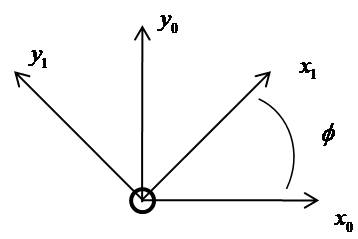
\includegraphics[width=5cm]{graphe1.jpg}}
\subfigure[rotation d'angle $\theta$]{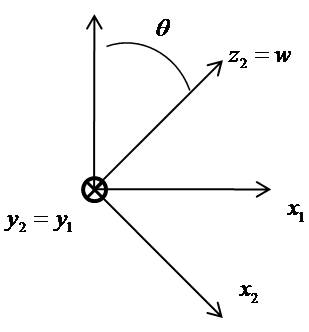
\includegraphics[width=5cm]{graphe2.jpg}}
\end{figure}

Pour positionner la caméra, on doit définir sa rotation propre autour de son axe optique. Pour cela on définit l'angle $\psi$ (figure \ref{decompositionGeometrique_rotationPropre}).
\begin{figure}[h!]
\centering
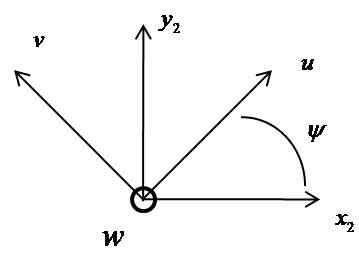
\includegraphics[width=5cm]{graphe3.jpg}
\caption{rotation propre}
\label{decompositionGeometrique_rotationPropre}
\end{figure}

On obtient alors 
\begin{equation*}
u=\cos(\psi)x_{2}+\sin(\psi)y_{2} \text{ et } v=-\sin(\psi)x_{2}+\cos(\psi)y_{2}
\end{equation*}
Si on pose $R_{s}$ la rotation d'angle $s$ et $\tau_{y}$ la translation de vecteur $-y$, on obtient alors 
\begin{equation*}
(\tau_{c}^{-1} \circ h)(X) = R_{\psi}\left(\frac{\delta (X_{v}-i(X))\cdot x_{2} }{w \cdot (X_{v}-i(X))+\delta'},\frac{\delta (X_{v}-i(X))\cdot y_{2}}{w \cdot (X_{v}-i(X))+\delta'}  \right) 
\end{equation*}
On assimile $X_{v}$ et $i^{-1}(X_{v})$ pour obtenir
\begin{equation*}
(R_{\psi}^{-1} \circ \tau_{c}^{-1}  \circ h)(X)=\delta \left(\frac{-i(\tau_{x_{v}} (X))\cdot x_{2} }{-w \cdot i(\tau_{x_{v}} (X))+\delta'},\frac{-i(\tau_{x_{v}} (X))\cdot y_{2}}{-w \cdot i(\tau_{x_{v}} (X))+\delta'}  \right) 
\end{equation*}

Comme $z_{2}=cos(\theta)z_{1}+sin(\theta)x_{1}$, $x_{2}=cos(\theta)x_{1}-sin(\theta)z_{1}$ et $z_{1}\perp P_{1}$, on a

\begin{equation*}
(R_{\psi}^{-1} \circ \tau_{c}^{-1}  \circ h)(X)=\delta\left(\frac{-\cos(\theta)i(\tau_{x_{v}} (X))\cdot x_{1} }{\delta'-\frac{sin(\theta)}{\delta'}x_{1}\cdot i(\tau_{x_{v}}(X))}, \frac{-i(\tau_{x_{v}} (X))\cdot y_{1}}{\delta'-\frac{sin(\theta)}{\delta'}x_{1}\cdot i(\tau_{x_{v}}(X))}  \right) 
\end{equation*}

En définissant $h_{\theta,\delta'}$ par

\begin{equation*}
h_{\theta,\delta'}(x',y')=\left(\frac{-cos(\theta)x'}{1-\frac{sin(\theta)}{\delta'}x'} ,\frac{-y'}{1-\frac{sin(\theta)}{\delta'}x'}\right)
\end{equation*}

Alors 

\begin{equation*}
(R_{\psi}^{-1} \circ \tau_{c}^{-1} \circ h)(X)= \frac{\delta}{\delta'}h_{\theta,\delta'}\left ( i(\tau_{x_{v}}(X)) \cdot x_{1}, i(\tau_{x_{v}}(X)) \cdot y_{1}\right)
\end{equation*}

Comme $x_{1}=\cos(\phi)x_{0}+\sin(\phi)y_{0}$ et $y_{1}=-\sin(\phi)x_{0}+\cos(\phi)y_{0}$, alors

\begin{eqnarray*}
(R_{\psi}^{-1} \circ \tau_{c}^{-1} \circ h)(X) &=& \frac{\delta}{\delta'}h_{\theta,\delta'}\left ( R_{\phi}(i(\tau_{x_{v}}(X)) \cdot x_{0}, i(\tau_{x_{v}}(X)) \cdot y_{0})\right)\\
                                               &=&\frac{\delta}{\delta'} (h_{\theta,\delta'}\circ R_{\phi} \circ \tau_{x_{v}})(X)
\end{eqnarray*}

Si on définit les dilatations $z_{\lambda}:X\rightarrow \lambda X$, alors on obtient la formule générale pour les mouvements de caméra
\begin{equation*}
h = \tau_{c} \circ z_{\frac{\delta}{\delta'}}  \circ R_{\psi} \circ h_{\theta,\delta'} \circ R_{\phi} \circ \tau_{x_{v}}
\label{formul_decomp}
\end{equation*}

\end{proof}



\subsubsection{Application à la décomposition des homographies :}
\paragraph{Résultats généraux sur les homographies :}
 On rappelle ici les notions sur les homographies qui nous seront utiles dans la suite. Le lien entre les homographies et les espaces projectifs ne sera pas étudié. Dans toute la suite du document, une homographie $h$ est une application bijective de la forme :
	\[h:(x,y)\mapsto \left(\frac{ax+by+p}{rx+sy+t},\frac{cx+dy+q}{rx+sy+t}\right)\]
(l'ensemble d'arrivée est $\mathbb R^2$ privé d'une droite).

Les applications affines sont un cas particulier d'homographie ; si une homographie n'est pas une application affine alors elle est définie sur le plan privé d'une droite appelée horizon.

L'ensemble des homographies a une structure de groupe pour la loi de composition.

On peut  associer à l'homographie $h$ la matrice $H$ définies par
  
\begin{equation*}
	H=\begin{pmatrix}
	a&b&p\\c&d&q\\r&s&t
	\end{pmatrix}
\end{equation*}
Cette matrice est inversible car $h$ est inversible, elle n'est pas unique car la matrice $\lambda H$ définit la même homographie pour $\lambda \in \mathbb{R}_+$.

Cette notation rend compatible le produit matriciel et la composition des homographies. On obtient un morphisme de groupe de $GL_{3}(\mathbb{R})$ dans le groupe des homographies du plan. Ce morphisme n'est pas injectif, la matrice d'une homographie est définie à proportionnalité près mais il se quotiente à travers $SL_{3}(\mathbb{R})$ en un isomorphisme.

Dans la suite on notera $\sim$ la relation d'équivalence  sur $GL_{3}(\mathbb{R})$ définie par $A\sim B \iff \exists \lambda\in \mathbb{R}^{*} , A=\lambda B$, c'est-à-dire si, et seulement si, $A$ et $B$ définissent la même homographie.

\underline{Remarque :} Dans certains cas une homographie peut être définie par ses valeurs prises en quatre points du plan.



\paragraph{Décomposition matricielle :}
\begin{prop}
Toute homographie est un mouvement de caméra avec un point visé ou une application affine. Dans le premier cas, la décomposition \ref{formul_decomp} n'est pas unique et possède un degré de liberté.
\end{prop}
%la ref n'apparait pas bien
\begin{proof}
On fixe $h$ une homographie et $H$ une matrice qui lui est associée. On conserve ici les notations de la partie précédente, on suppose sans perte de généralité que $\det (H)=1$. On suppose de plus que $h$ peut s'écrire sous la forme $\ref{formul_decomp}$, on cherche à montrer que cette hypothèse n'impose aucune condition supplémentaire sur la matrice $H$, en déterminant les paramètres intervenants dans la décomposition en fonction des coefficients de $H$ .

On a la formule de décomposition :

\begin{equation*}
h= \tau_{c} \circ z_{\frac{\delta}{\delta'}}\circ R_{\psi} \circ h_{\theta,\delta'} \circ R_{\phi} \circ \tau_{x_{v}}
\end{equation*}
Chacune de ces transformations est une homographie, on peut donc réécrire cette relation en utilisant des matrices. On obtient 
 \begin{equation*}
H\sim T_{c} Z_{\frac{\delta}{\delta'}}  R_{\psi}  H_{\theta,\delta'} R_{\phi}  T_{x_{v}}
\end{equation*}
avec
\begin{equation*}
R_{\alpha}=\begin{pmatrix}
\cos(\alpha)&\sin(\alpha)&0\\-\sin(\alpha)&cos(\alpha)&0\\0&0&1
\end{pmatrix}
, H_{\theta,\delta'}=\begin{pmatrix}
-\cos(\theta)&0&0\\0&-1&0\\-\frac{\sin(\theta)}{\delta'}&0&1
\end{pmatrix},
\end{equation*}
\begin{equation*}
Z_{\lambda}=\begin{pmatrix}
\lambda&0&0\\0&\lambda&0\\0&0&1
\end{pmatrix}
\text{ et } T_{X_{v}}=\begin{pmatrix}
1&0&-x_{v}\\0&1&-y_{v}\\0&0&1
\end{pmatrix}
\end{equation*}
 On cherche dans un premier temps à déterminer les translations. Soient $X_1 = (x_1 , y_1 )$ et $X_2 = (x_2 , y_2 )$ deux vecteurs que l'on suppose tel que la matrice $H_t$ définie par $H_t = T_{-X_2}  \cdot H \cdot T_{X_1}$ admette une décomposition de la forme  $H_t=R_{\psi} \cdot H_{\theta,\delta} \cdot R_{\phi}$.
 
 On notera
 \begin{equation*}
 H^{-1}=\begin{pmatrix} \hat a&\hat b&\hat p\\ \hat c&\hat d&\hat q\\ \hat r&\hat s&\hat t \end{pmatrix}
 \end{equation*}
 Par un calcul on obtient que la matrice $R_{\psi} \cdot H_{\theta,\delta} \cdot R_{\phi}$ est égale à : 
  \begin{equation*}
\begin{pmatrix}
 -\frac{\delta}{\delta'}\cos(\psi)\cos(\theta)\cos(\phi)+\frac{\delta}{\delta'}\sin(psi)\sin(\phi)& -\frac{\delta}{\delta'}\cos(\psi)\cos(\theta)\sin(\phi)-\frac{\delta}{\delta'}\sin(\psi)\cos(\phi)&0\\
  \frac{\delta}{\delta'}\sin(\psi)\cos(\theta)\cos(\phi)+\frac{\delta}{\delta'}\cos(\psi)\sin(\phi)& \frac{\delta}{\delta'}\sin(\psi)\cos(\theta)\sin(\phi)-\frac{\delta}{\delta'}\cos(\psi)\cos(\phi)&0\\ -\frac{\sin(\theta)}{\delta'}\cos(\phi)&-\frac{\sin(\theta)}{\delta'}\sin(\phi)& 1
 \end{pmatrix}
 \end{equation*}
 On a de plus 
 \begin{equation*}
 H_t=\begin{pmatrix}
 a-x_2 r&b-x_2 s& a x_1 + b y_1 + p -x_2 (r x_1 +s y_1 +t)\\
  c-y_2 r&d-y_2 s& c x_1 + d y_1 + q -y_2 (r x_1 +s y_1 +t)\\
  r & s & r x_1 + s y_1 +t
 \end{pmatrix}
 \end{equation*}
 On a donc l'équivalence 
 \begin{equation*}
 (H_t)_{1,3}=(H_t)_{2,3}=0 \iff (x_2,y_2)=h(x_1,y_1) \iff (x_1,y_1)=h^{-1}(x_2,y_2)
 \end{equation*}
 On pose $(x_1,y_1)=h^{-1}(x_2,y_2)$ car les calculs intermédiaires sont moins fastidieux, on suppose $(x_2,y_2)$ tels que $\hat r x_2 +\hat s y_2 + \hat t \ne 0$.\\
On obtient alors
\begin{equation*}
H_t
  \sim 
  \begin{pmatrix}
 (a-x_2 r)(\hat r x_2 + \hat s y_2 +\hat t)&(b-x_2 s)(\hat r x_2 + \hat s y_2 +\hat t)& 0\\
  (c-y_2 r)(\hat r x_2 + \hat s y_2 +\hat t)&(d-y_2 s)(\hat r x_2 + \hat s y_2 +\hat t)& 0\\
  r(\hat r x_2 + \hat s y_2 +\hat t) & s(\hat r x_2 + \hat s y_2 +\hat t) &1
  \end{pmatrix} 
\end{equation*}
On obtient alors 
 \begin{equation*}
 -\frac{\sin(\theta)}{\delta'}\cos(\phi)=r(\hat r x_2 + \hat s y_2 +\hat t)\text{ et } -\frac{\sin(\theta)}{\delta'}\sin(\phi)=s(\hat r x_2 + \hat s y_2 +\hat t)
 \end{equation*}
 On sait que $r^{2}+s^{2}=0$ si et seulement si l'homographie associée à H est une affinité. Ce cas ci sera traité de façon indépendante, on suppose ici que l'homographie $h$ n'est pas une affinité. On peut donc écrire :
 \begin{eqnarray*}
 \cos(\psi) &=& \sgn\left(-\frac{\sin(\theta)}{ \delta'}\right)\sgn(\hat r x_2 + \hat s y_2 +\hat t)\frac{r}{\sqrt{r^{2}+s^{2}}}\\
 \sin(\psi) &=& \sgn\left(-\frac{\sin(\theta)}{ \delta'}\right)\sgn(\hat r x_2 + \hat s y_2 +\hat t)\frac{s}{\sqrt{r^{2}+s^{2}}}
 \end{eqnarray*}
 On peut se restreindre au cas $\frac{\sin(\theta)}{\delta'}>0$ :\\
 \begin{itemize}
 \item En effet si $\frac{\sin(\theta)}{\delta'}<0$ on obtient alors
 \begin{equation*}
 R_{\psi} \cdot H_{\theta,\delta'} \cdot R_{\phi}=R_{\psi} \cdot Z_{-1}\cdot H_{\theta,-\delta'}\cdot Z_{-1} \cdot R_{\phi}= R_{\psi+\pi} \cdot H_{\theta,-\delta'}\cdot R_{\phi+\pi}
 \end{equation*}
 et on a $-\frac{\sin(\theta)}{\delta'}>0$.\\
 \end{itemize}


 On obtient alors 
 \begin{equation*}
 \cos( \phi )= -\sgn(\hat r x_2 +\hat s y_2 +\hat t) \frac{r}{\sqrt{r^2 + s^2}} \text{ et } \sin( \phi )= -\sgn(\hat r x_2 +\hat s y_2 +\hat t) \frac{s}{\sqrt{r^2 + s^2}}
 \end{equation*}
 Comme 
 \begin{equation*}
H_t \cdot R_{\phi}^{-1} \sim
 \begin{pmatrix}
 -|\hat r x_2 +\hat s y_2 +\hat t|\frac{(ar+sb)-(r^2 + s^2)x_2}{\sqrt{r^2 + s^2}}&-|\hat r x_2 +\hat s y_2 +\hat t|\frac{\hat s}{\sqrt{r^2 + s^2}}&0\\
 -|\hat r x_2 +\hat s y_2 +\hat t|\frac{(cr+sd)-(r^2 + s^2)y_2}{\sqrt{r^2 + s^2}}&|\hat r x_2 +\hat s y_2 +\hat t|\frac{r}{\sqrt{r^2 + s^2}}&0\\
 -|\hat r x_2 +\hat s y_2 +\hat t|\sqrt{r^2 + s^2}&0&1
 \end{pmatrix}
 \end{equation*}
 Et d'un autre côté 
 \begin{equation*}
R_{\psi} \cdot H_{\theta,\delta}  \sim 
 \begin{pmatrix}
 -\frac{\delta}{\delta'}\cos(\psi)\cos(\theta)&
-\frac{\delta}{\delta'}\sin(\psi)&
0\\
\frac{\delta}{\delta'}\sin(\psi)\cos(\theta)&
-\frac{\delta}{\delta'}\cos(\psi)&
0\\
-\frac{\sin(\theta)}{\delta'}&
0&
1
 \end{pmatrix}
 \end{equation*}
Comme $h$ n'est pas une affinité on a $\hat r^2 + \hat s^2 \ne 0$ 
 \begin{equation*}
  \cos( \psi ) =- \sgn(\frac{\delta}{\delta'})\frac{\hat r}{\sqrt{\hat r^2 + \hat s^2}}\text{ et } \sin( \psi ) = \sgn(\frac{\delta}{\delta'})\frac{\hat s}{\sqrt{\hat r^2 + \hat s^2}}
 \end{equation*}
On peut se restreindre au cas $\frac{\delta}{\delta'}>0$ :\\
\begin{itemize}
\item En effet si $\frac{\delta}{\delta'}<0$ on obtient alors $Z_{\frac{\delta}{\delta'}} \cdot R_{\psi}=Z_{\left|\frac{\delta}{\delta'}\right|}\cdot Z_{-1} \cdot R_{\psi}=Z_{\left|\frac{\delta}{\delta'}\right|}\cdot R_{\pi} \cdot R_{\psi}=Z_{\left|\frac{\delta}{\delta'}\right|}\cdot R_{\psi+\pi}$.
\end{itemize}
Et donc 
 \begin{equation*}
  \cos( \psi ) =- \frac{\hat r}{\sqrt{\hat r^2 + \hat s^2}} \text{ et } \sin( \psi ) = \frac{\hat s}{\sqrt{\hat r^2 + \hat s^2}}
 \end{equation*}



 On obtient alors 
\begin{equation*}
R_{\psi}^{-1} \cdot H_t \cdot R_{\phi}^{-1} \sim 
 \begin{pmatrix}
 -|\hat r x_2 +\hat s y_2 +\hat t|(\hat r x_2 +\hat s y_2 +\hat t)\sqrt{\frac{r^2 + s^2}{\hat r^2 + \hat s^2}}&0&0\\
 |\hat r x_2 +\hat s y_2 +\hat t|\frac{\Delta_H(x_2 , y_2)}{\sqrt{r^2 + s^2}\sqrt{\hat r^2 + \hat s^2}}&-|\hat r x_2 +\hat s y_2 +\hat t|\sqrt{\frac{\hat r^2 + \hat s^2}{r^2 + s^2}}&0\\
 -|\hat r x_2 +\hat s y_2 +\hat t|\sqrt{r^2 + s^2}&0&1
 \end{pmatrix}
\end{equation*}
Où l'on a posé 
\begin{equation*}
\Delta_H(x_2 , y_2 ) =\hat r ((rc+sd)-(r^2 + s^2)y_2) - \hat s ((ar+sb)-(r^2 + s^2 )x_2)
\end{equation*}
Les solutions de $\Delta_H(x_2 , y_2 )=0$ sont
\[ \left\lbrace \left( x_2=\frac{ar+sb+ \hat r \lambda}{r^2 +s^2}, y_2=\frac{cr+sd+\hat s \lambda}{r^2 +s^2}\right), \lambda \in \mathbb R \right\rbrace\]
On a dans ce cas
\begin{equation*}
\hat r x_2 +\hat s y_2 +\hat t = \frac{\hat r^2 +\hat s^2}{r^2 + s^2} \lambda
\end{equation*}
Le paramètre $\lambda$ doit donc être pris différent de zéro car 
\begin{equation*}
R_{\psi}^{-1} \cdot H_t \cdot R_{\phi}^{-1} \sim 
 \begin{pmatrix}
 -| \lambda | \lambda \sqrt{\frac{\hat r^2 + \hat s^2}{s^2 + r^2}}^{3}&0&0\\
0&-| \lambda | \sqrt{\frac{\hat r^2 + \hat s^2}{r^2 + s^2}}^{3}&0\\
 -|\lambda|\frac{\hat r^2 + \hat s^2}{\sqrt{r^2 + s^2}}&0&1
 \end{pmatrix}
\end{equation*}
 
 
 On peut poser 
 \begin{equation*}
 \frac{\delta}{\delta'}=|\lambda|\sqrt{\frac{\hat r^2 + \hat s^2}{r^2 + s^2}}^{3}
 \end{equation*}
On obtient finalement
\begin{equation*}
Z_{\frac{\delta}{\delta'}}^{-1} \cdot R_{\psi}^{-1} \cdot H_t \cdot R_{\phi}^{-1} \sim 
 \begin{pmatrix}
 -\lambda&0&0\\
0&-1&0\\
 -|\lambda|\frac{\hat r^2 + \hat s^2}{\sqrt{r^2 + s^2}}&0&1
 \end{pmatrix}
 \end{equation*}
 Cette matrice doit être de la forme $H_{\theta,\delta'}$. Pour qu'elle le soit, on doit avoir 
 \begin{equation*}
  \lambda^2 + \lambda^2 \delta'^2 \frac{(\hat r^2 + \hat s^2)^2}{r^2 + s^2}=1
 \end{equation*}
 C'est-à-dire
 \begin{equation*}
  \delta'^2 = (r^2 + s^2) \frac{1-\lambda^2}{\lambda^2 (\hat r^2+\hat s^2)^2}
 \end{equation*}
\end{proof}
 %\paragraph{Synthèse et optimisation :}
 %On a montré dans la section précédente que toute homographie qui n'est pas une application affine est un mouvement de caméra. On a de plus que pour tout $\lambda \in ]0,1[$ %pas certain que c'est ce que tu veux dire
 %\begin{equation*}
%x_2=\frac{ar+sb+\hat r \lambda}{r^2 +s^2}, y_2=\frac{cr+sd+\hat s \lambda}{r^2 +s^2}, (x_1 , y_1) = h^{-1}(x_{2},y_{2})
%\end{equation*}
 %\begin{equation*}
 %\cos( \phi )= - \frac{r}{\sqrt{r^2 + s^2}},  \sin( \phi )= - \frac{s}{\sqrt{r^2 + s^2}}, \cos( \psi ) =- \frac{\hat r}{\sqrt{\hat r^2 + \hat s^2}},  \sin( \psi ) = \frac{\hat s}{\sqrt{\hat r^2 + \hat s^2}}
 %\end{equation*}
 %\begin{equation*}
 %\frac{\delta}{\delta'}=|\lambda|\sqrt{\frac{\hat r^2 + \hat s^2}{r^2 + s^2}}^{3}, \cos(\theta)=\lambda, \sin(\theta)=\sqrt{1-\lambda^2}, \delta'=  \frac{\sqrt{(r^2 + s^2)(1-\lambda^2)}}{|\lambda| (\hat r^2+\hat s^2)}
 %\end{equation*}
 %Le degré de liberté correspond à une translation en sortie dans une direction perpendiculaire à l'horizon de $H^{-1}$.\\
 %Une décomposition plus générale autorise $\lambda \in \mathbb{\hat r}^{*}$.
%

 \paragraph{Synthèse et utilisation :}
  On a donc montré que toute homographie (autre qu'une affinité) peut s'identifier à un mouvement de caméra. Plus précisément, pour tout $\lambda \in ]0,1[$,

  \begin{equation*}
H \sim T_{c} Z_{\frac{\delta}{\delta'}}  R_{\psi}  H_{\theta,\delta'} R_{\phi}  T_{x_{v}}
  \end{equation*}
  avec $T_c$ translation de vecteur $(x_2,y_2)$, $T_{x_v}$ translation envoyant $(0,0)$ sur le point visé $X_v$, et
 \begin{equation*}
x_2=\frac{ar+sb+\hat r \lambda}{r^2 +s^2}, y_2=\frac{cr+sd+\hat s \lambda}{r^2 +s^2}, (x_1 , y_1) = h^{-1}(x_{2},y_{2})
  \end{equation*}
 \begin{equation*}
 \cos( \phi )= - \frac{r}{\sqrt{r^2 + s^2}}, \sin( \phi )= - \frac{s}{\sqrt{r^2 + s^2}},\cos( \psi ) =- \frac{\hat r}{\sqrt{\hat r^2 + \hat s^2}}, \sin( \psi ) = \frac{\hat s}{\sqrt{\hat r^2 + \hat s^2}}
 \end{equation*}
 \begin{equation*}
 \frac{\delta}{\delta'}=|\lambda|\sqrt{\frac{\hat r^2 + \hat s^2}{r^2 + s^2}}^{3}, \cos(\theta)=\lambda, \sin(\theta)=\sqrt{1-\lambda^2}, \delta'=  \frac{\sqrt{(r^2 + s^2)(1-\lambda^2)}}{|\lambda| (\hat r^2+\hat s^2)}
 \end{equation*}
 Le degré de liberté $\lambda$ correspond à une translation en sortie dans une direction perpendiculaire à l'horizon de $H^{-1}$.
 
 On peut commuter $Z_{\frac{\delta}{\delta'}}$ et $R_{\psi}$, et introduire une translation $T'$ telle que $R_{\phi}  T_{x_{v}} = T' R_\phi$. On arrive donc à une décomposition
   \begin{equation*}
H \sim T_{c} R_{\psi}  \tilde H R_{\phi}
  \end{equation*}
  Les affinités $T_{c} R_{\psi}$ et $R_{\phi}$ sont des isométries, et même principalement des rotations (la translation pouvant être prise en compte en considérant qu'on change l'endroit du plan traité). Il existe donc déjà des manières efficaces de les traiter (étudiée en \ref{YaroSzeli}).
  
  L'homographie $\tilde H$ est une homographie de la forme
  \[\tilde H = \pmatrice{*&0&*\\ 0&*&*\\ *&0&*}\]
  qui est une forme particulière permettant d'être plus facilement qu'une homographie quelconque (voir \ref{HomoboxRipmap}).
  
 Formellement, on peut s'autoriser $\lambda \in \mathbb R^*$ ; la décomposition matricielle reste alors correcte, mais elle perd son interprétation géométrique ($\lambda$ ne peut plus être identifié à un cosinus). De plus, on peut prendre $\phi + \pi$ au lieu de $\phi$ (de même pour $\psi$), car cela aura uniquement pour effet de multiplier certains coefficients de $\tilde H$ par $-1$.
 
 On en déduit donc un traitement d'une homographie générale, non affine, en passant par deux rotations-translations et une homographie particulière, correspondant à l'algorithme \ref{pseudoCodeDecompo}. Le traitement des affinités et des homographies correspond aux deux prochaines parties.
		
	\begin{figure}
		\centering
		\subfigure[Vue de départ]{
		{
\includegraphics[width=60mm]{vue_fps_identity.png}}
		{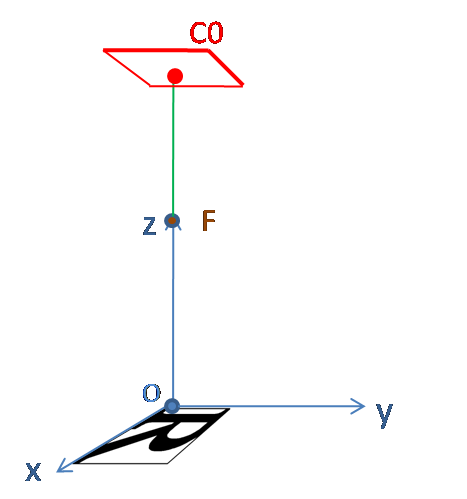
\includegraphics[scale=0.5]{vue_tps_identity.png}}}\\
		\subfigure[Vue après une première rotation (d'angle $\phi$)]{
		{
\includegraphics[width=60mm]{vue_fps_rotation_phi.png}}
		{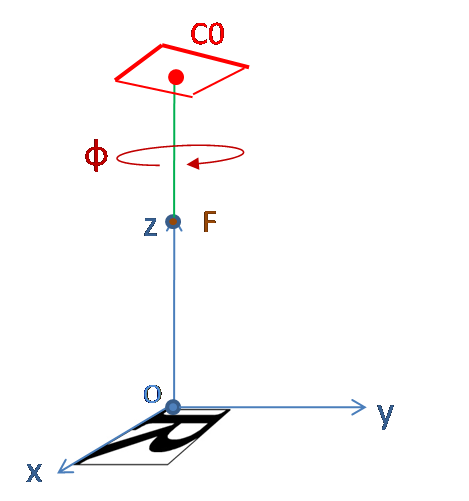
\includegraphics[scale=0.5]{vue_tps_rotation_phi.png}}}\\
		\subfigure[Vue après l'homographie particulière]{
		{
\includegraphics[width=60mm]{vue_fps_hom_part.png}}
		{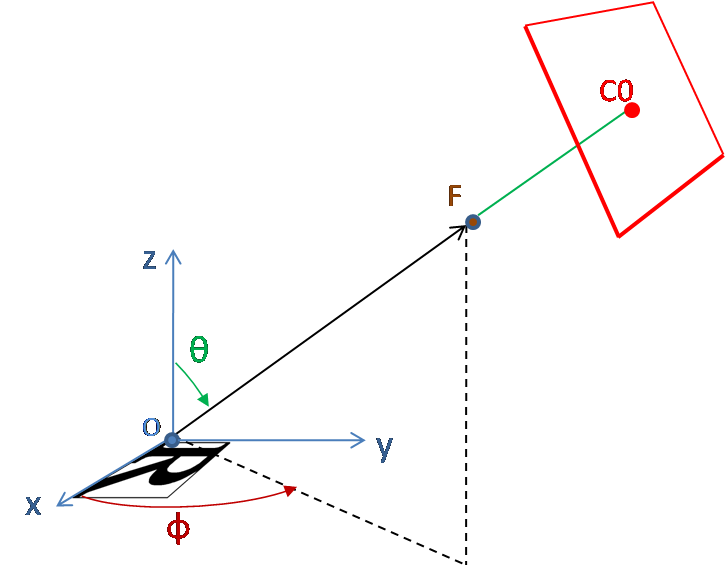
\includegraphics[scale=0.5]{vue_tps_hom_part.png}}}\\
		\subfigure[Vue finale (après rotation d'angle $\psi$)]{
		{
\includegraphics[width=60mm]{vue_fps_rotation_psi.png}}
		{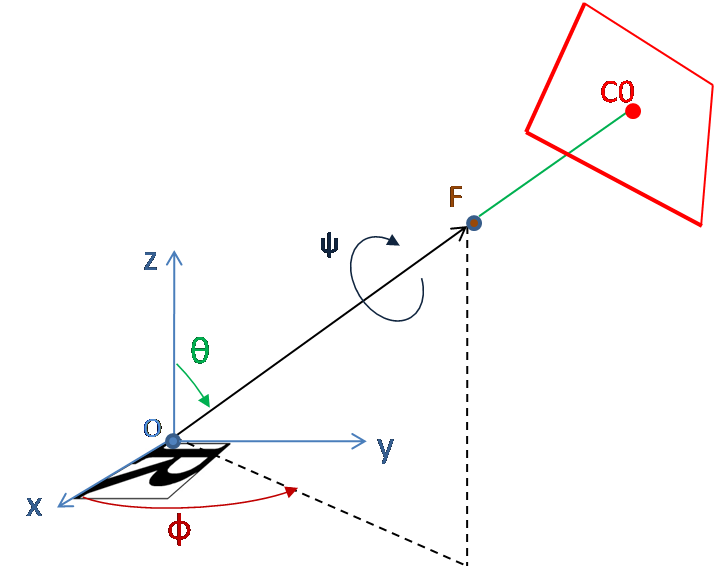
\includegraphics[scale=0.5]{vue_tps_rotation_psi.png}}}
		\caption{Étapes de traitement d'une homographie, assimilées à des mouvements de caméra (à gauche la vue de la caméra, à droite une vue extérieure immobile). Sur les vues extérieures, $F$ représente le point focal de la caméra, le plan rouge est le plan image de la caméra}
	\end{figure}
